%%%%%%%%%%%%% You can ignore this stuff
\documentclass[bsc]{abdnthesis}
\usepackage[linktocpage=true,hidelinks]{hyperref}

\usepackage[T1]{fontenc}
\usepackage[utf8]{inputenc}
\usepackage{booktabs}
\usepackage{longtable}
\usepackage{csquotes}
\usepackage[acronym]{glossaries}
\usepackage[automake]{glossaries-extra}
\newglossarystyle{modsuper}{%
  \glossarystyle{super}%
  \renewcommand{\glsgroupskip}{}
}
\makeglossaries


\usepackage[style=apa, backend=biber, natbib=true]{biblatex}
\DefineBibliographyStrings{english}{%
  bibliography = {References},
}

\addbibresource{refs.bib}

% This creates hyperlinks and moves the contents links to the page number for clarity

\def\subsectionautorefname{Section}
\def\subsubsectionautorefname{Section}
\def\sectionautorefname{Section}
\def\chapterautorefname{Chapter}

%%%%%%%%%%%%%%%%% Space for your own packages here %%%%%%%%%%%%%%%%%%%%%%%%%%%%%%
% Uncomment for blank lines between paragraphs rather than
% indents
\usepackage[parfill]{parskip}
\usepackage{xcolor} %Great if you want coloured text
\usepackage{algorithm}
\usepackage{algorithmic} %Algorithm styles, need to be nested for the example shown
\usepackage{graphicx,color}
\usepackage{listings}
\graphicspath{ {./images/} }

\hypersetup{linktocpage}
\hypersetup{
  linktoc=all,     %set to all if you want both sections and subsections linked
}

\definecolor{codegreen}{rgb}{0,0.6,0}
\definecolor{codegray}{rgb}{0.5,0.5,0.5}
\definecolor{codepurple}{rgb}{0.58,0,0.82}
\definecolor{backcolour}{rgb}{0.95,0.95,0.92}

\definecolor{lightgray}{rgb}{.9,.9,.9}
\definecolor{darkgray}{rgb}{.4,.4,.4}
\definecolor{purple}{rgb}{0.65, 0.12, 0.82}

\lstdefinelanguage{JavaScript}{
  keywords={typeof, new, true, false, catch, function, return, null, catch,
      switch, var, if, in, while, do, else, case, break},
  keywordstyle=\color{blue}\bfseries,
  ndkeywords={class, export, boolean, throw, implements, import, this},
  ndkeywordstyle=\color{darkgray}\bfseries,
  identifierstyle=\color{black},
  sensitive=false,
  comment=[l]{//},
  morecomment=[s]{/*}{*/},
  commentstyle=\color{purple}\ttfamily,
  stringstyle=\color{red}\ttfamily,
  morestring=[b]',
  morestring=[b]',
}

\lstdefinestyle{normal}{
  backgroundcolor=\color{backcolour},
  commentstyle=\color{codepurple},
  keywordstyle=\color{magenta},
  numberstyle=\tiny\color{codegray},
  stringstyle=\color{codegreen},
  basicstyle=\ttfamily\footnotesize,
  breakatwhitespace=false,
  breaklines=true,
  captionpos=b,
  keepspaces=true,
  numbers=left,
  numbersep=5pt,
  showspaces=false,
  showstringspaces=false,
  showtabs=false,
  tabsize=2
}
\lstdefinestyle{php}{
  backgroundcolor=\color{backcolour},
  commentstyle=\color{codepurple},
  keywordstyle=\color{magenta},
  numberstyle=\tiny\color{codegray},
  stringstyle=\color{codegreen},
  basicstyle=\ttfamily\footnotesize,
  otherkeywords={with},
  breakatwhitespace=false,
  breaklines=true,
  captionpos=b,
  keepspaces=true,
  numbers=left,
  numbersep=5pt,
  showspaces=false,
  showstringspaces=false,
  showtabs=false,
  tabsize=2
}

\lstdefinestyle{python}{
  backgroundcolor=\color{backcolour},
  commentstyle=\color{codepurple},
  keywordstyle=\color{magenta},
  numberstyle=\tiny\color{codegray},
  stringstyle=\color{codegreen},
  basicstyle=\ttfamily\footnotesize,
  otherkeywords={with},
  breakatwhitespace=false,
  breaklines=true,
  captionpos=b,
  keepspaces=true,
  numbers=left,
  numbersep=5pt,
  showspaces=false,
  showstringspaces=false,
  showtabs=false,
  tabsize=2
}

%%%%%%%%%%%%%%%%%%%%%%%%%%%%%%%%%%%%%%%%%%%%%%%%%%%%%%%%%%%%%%%%%%%%%%%%%%%%%%%%%

\title{A Web Driven SDN Orchestrator For The Provisioning of ACI Fabric and Lab
  Infrastructure}
\author{Matthew Gaynor}
\upnumber{922830}

\projecttype{Engineering Project}
\school{School of Computing}

%%%% In the final submission of a thesis, this should only be the year
%%%% of submission.  However, it is useful to use \date{\today} for drafts so that
%%%% they don't get mixed up.

\date{2023}

%% It is useful to split the document up as chapters and include
%% them.  LaTeX will sort out all the numbering and cross-referencing
%% for you --- if you run it enough times!

\begin{document}

%%%% Create the title page and standard declaration.

\maketitle
\makedeclaration

%%%% Then the abstract and acknowledgements

\newacronym{svs}{SVS}{Solution Validation Services}
\newacronym{cli}{CLI}{Command Line Interface}
\newacronym{cx}{CX}{Customer Experience}
\newacronym{dmz}{DMZ}{Demilitarised Zone}
\newacronym{wan}{WAN}{Wide Area Network}
\newacronym{vpn}{VPN}{Virtual Private Network}
\newacronym{nos}{NOS}{Network Operating System}
\newacronym{fex}{FEX}{Fabric Extender}
\newacronym{tor}{ToR}{Top of Rack}
\newacronym{dpg}{DPG}{Distrubited Port Group}
\newacronym{dvs}{DVS}{Distributed Virtual Switch}
\newacronym{ntp}{NTP}{Network Time Protocol}
\newacronym{dns}{DNS}{Domain Name System}
\newacronym{radius}{RADIUS}{Remote Authentication Dial-In User Service}
\newacronym{aci}{ACI}{Application Centric Infrastructure}
\newacronym{spa}{SPA}{Singple Page Application}
\newacronym{api}{API}{Application Programming Interface}
\newacronym{rest}{REST}{Representational State Transfer}
\newacronym{orm}{ORM}{Object Relational Mapping}
\newacronym{http}{HTTP}{HyperText Transfer Protocol}
\newacronym{mvc}{MVC}{Model View Controller}
\newacronym{erd}{ERD}{Entity Relationship Diagram}
\newacronym{apic}{APIC}{Application Policy Infrastructure Controller}
\newacronym{oob}{OOB}{Out of Band}
\newacronym{nat}{NAT}{Network Address Translation}
\newacronym{vm}{VM}{Virtual Machine}
\newacronym{vrf}{VRF}{Virtual Routing and Forwarding}
\newacronym{epg}{EPG}{Endpoint Group}
\newacronym{ddi}{DDI}{DNS, DHCP and IP Address Management (IPAM)}
\newacronym{bd}{BD}{Bridge Domain}
\newacronym{ospf}{OSPF}{Open Shortest Path First}
\newacronym{mp-bgp}{MP-BGP}{Multi-Protocol Border Gateway Protocol}
\newacronym{as}{AS}{Autonomous System}
\newacronym{ssh}{SSH}{Secure Shell}
\newacronym{vpc}{vPC}{Virtual Port Channel}
\newacronym{aaep}{AAEP}{Attachable Access Entity Profile}
\newacronym{lacp}{LACP}{Link Aggregation Control Protocol}
\newacronym{svi}{SVI}{Switch Virtual Interface}
\newacronym{dhcp}{DHCP}{Dynamic Host Configuration Protocol}
\newacronym{acl}{ACL}{Access Control List}
\begingroup     
\let\clearpage\relax
\glsaddall
\printglossary[style=modsuper, type=\acronymtype, nonumberlist, nopostdot, title=Abbreviations] 
\endgroup
\section*{Abstract}
This project will aim to provide an automation platform to CX Labs UK within Cisco Systems that will streamline DMZ lab operations by providing a web interface that will allow infrastructure to be managed from the perspective of the available rackspace. Cisco Application Centric Infrastructure shall be used to provide network connectivity and VMware ESXi and vCenter shall be used to provide compute resources. A testbed will be constructed to emulate a scaled-down version of lab infrastructure that will be used to develop and test the automation platform against Cisco ACI and vCenter. The platform will aim to obfuscate as much network configuration as possible, resulting in a drastic reduction in time spent provisioning lab rackspace when a project enters or terminates. This will result in a streamlined network configuration that represents the current state of usage, as the configuration will be managed entirely by the automation platform and derived from the users inputs into the web interface.



Word Count: 11111
\section*{Acknowledgements}
I would like to thank Cisco, my manager and good friend, Dave Smith, for his
close help in allowing me to use equipment necessary for testing and developing the solution.
\section*{Consent to Share}
I consent for this project to be archived by the University
Library and potentially used as an example project for future students.



%% please indicate whether you are happy for other students to
%% view your project in the future

%%%% These are macros ( each macro is defined by \newcommand )
%%%% These macros make cross-referencing easier, building on the
%%%% already very useful \autoref{ref}.  You tweak them or build your own.

%% \autorefp{ref}
%% Like \autoref, but adds the page number
%% e.g. Section 3.2.4 (p345)
\newcommand{\autorefp}[1]{\autoref{#1} (p\pageref*{#1})}

%% \autorefnp{ref}
%% Like \autoref, but adds both the section name and page number
% e.g. Section 3.2.4 "blah blah" (p345)
\newcommand{\autorefnp}[1]{\autoref{#1} ``\nameref{#1}'', (p\pageref*{#1})}

%% \see{ref}
%% Handy shorthand for inserting a hyperlinked xref.
%%   e.g. (see Section 3.2.4, p134)
%%        (see Figure 5.1, p23)
%%        (see Table 4.7, p999)
\newcommand{\see}[1]{\hyperref[#1]{(see \autoref*{#1}, p\pageref*{#1})}}

%% \seenamed{ref}
%% Handy shorthand for inserting a hyperlinked xref that also includes
%% the name of the section being referred to.
%% (see Section 3.2.4 "blah blah", p134)
%% (see Figure 5.1 "blah blah blah!", p23)
%% (see Table 4.7 "blah blah blah blah blah blah", p999)
\newcommand{\seenamed}[1]{\hyperref[#1]{(see \autoref*{#1} ``\nameref*{#1}'',
    p.\pageref*{#1})}}

%% \bq Block Quotations.
\newcommand{\bq}[2][]{\singlespacing \begin{quote}
    \begin{small} ``\textit{#2}'' \end{small} #1 \end{quote} \doublespacing}

%% \qq{quotation}
%% Shortcut for doing inline quotations (with 6699 quotation marks around italic text)
%% e.g. \qq{To be, or not to be}
\newcommand{\qq}[1]{{\enquote{\textit{#1}}}}

%%%% It should have a table of contents, but delete the other two as
%%%% necessary.

\tableofcontents
\listoftables
\listoffigures

\chapter{Introduction}
\label{chap:intro}

\section{The Client}
\label{intro:client}
This project will be developed with the intention of it
being utilised by a client, for the benefit of their operation.
The client is
CX Labs UK within Cisco Systems. CX Labs provides lab space for
use by business
units internal to the company. Most of the space is used for
the testing of
customer networks by SVS (Solution Validation Services). SVS
provides bespoke
testing services to customers wishing to use Cisco’s expertise
to test a range
of scenarios, from regression and firmware testing to full
upgrade and
migration plans.\newline
To match the customer's environment as close as
possible, a scaled-down
version of the customer's network is usually recreated
in the lab space managed
by CX Labs. CX Labs hold many devices that cover most
of the Cisco portfolio,
which allows for the recreation of most networks. Most
of this lab space is
hosted within the internal Cisco corporate network which
requires any users to
be employees of Cisco to access testbeds. More and more
customers
however are requesting remote access to their testbeds so they can
perform their own testing. To facilitate this, a
fully isolated DMZ environment
is provided, which allows direct WAN
connectivity to a testbed, allowing for a
VPN tunnel to be established and
hence remote access granted to a testbed from
any location to any permitted
person.

\subsubsection{Current Infrastructure}
The current infrastructure to support the testbeds consists of four Nexus 9K
core switches, with \gls{fex}s to provide copper connectivity. Currently, the
N9Ks do not have any form of \gls{vpc} configured, and just use \gls{stp} for
redundancy. \gls{tor} connectivity is provided by Catalyst switches. Each
project has a dedicated VLAN to isolate communications between different
projects, and a virtual router and services stack is hosted on a vCenter
environment to provide internet and \gls{vpn} connectivity to the project. Each
project also has several terminal servers attached to its VLAN so that the
console ports of the testbed devices can be easily accessed in case of a device
problem.

\subsubsection{Current Project Pipeline}
When a new testbed build is
requested, the project topology is reviewed, which will indicate how much
rackspace will be required to accommodate the project. Suitable racks will then
be chosen to house the project based on cooling, power and space requirements.
A new VLAN for the project will then be manually created across all of the
associated networking equipment, including the core N9Ks, and the \gls{tor}
switches that live in the selected racks. Terminal servers will also have to be
reconfigured so that they have the correct subnet configured and the correct
sub-interface configured. The next step is to provision a virtual CSR1000v
router hosted on vCenter that will provide \gls{nat} and internet access to the
newly created VLAN. A services stack will then be deployed to take care of
remote access \gls{vpn} and other associated services. Both of these steps
require the manual addition of a \gls{dpg} to the \gls{dvs} present in vCenter.
\section{The Problem}
\label{intro:problem}
Whilst the existing solution does
function, several problems frequently arise which reduce the operational
efficiency of the lab:

A large initial time investment is required when
onboarding a new project. This is due to the manual configuration of the
networking equipment, as well as the manual deployment of the virtual router
and services stack. This time could be better spent on other tasks, such as
preparing the physical rackspace for the racking and stacking of new equipment.

No configuration management system is in place, which results in configuration
drift over time. When projects are removed, the configuration is sometimes
inconsistently modified on devices. Both VLANs and \gls{dpg}s become
unsynchronised and often differ between the core switches themselves, resulting
in confusion when modifying configuration. In the past, this has led to
accidental removal and modification of configuration related to other projects,
which impacts customer availability and takes time away from the team that
could otherwise have been used to tackle other issues.

No centralised device
management is utilised which results in device health and firmware being hard to update and monitor.
This is because each device has to be manually updated, which is a
time-consuming process. This also means that the devices are not all running
the same version of firmware, which can cause issues when troubleshooting. A
lack of centralised management makes device failure also hard to detect as there is no
centralised monitoring solution in place, so reports from the testing team or
customer are often the first indication that a problem has arisen.

\section{Aims and Objectives}
\label{intro:aims}

This project aims to provide
a solution that will automate the
configuration of the DMZ network
infrastructure, as well as the configuration of the associated project
infrastructure, such as the project router, services stack and terminal
servers. This will be achieved by providing a web-based dashboard that allows
the user to provision a new project, which will then automatically configure
the required infrastructure. The solution will revolve around recreating the
physical rackspace inside the web interface. The concept behind this is a
one-to-one mapping between the real-world rackspace and the virtual rackspace.
The virtual rack can then have the \gls{tor} and terminal server that resides
in the real-world rack associated with it. A project can then be allocated
virtual racks and have the associated infrastructure that is tied to a rack
automatically provisioned. The solution will also provide a view of the current
utilisation of the lab space by projects, as well as the current utilisation of
the lab space as a whole.

The solution will use Cisco \gls{aci} to provide
network connectivity. This removes the complexities that would otherwise be
associated with provisioning many network devices via \gls{ssh} or RESTCONF.
\gls{aci} will also make the network highly scalable, with the ability to add
additional leafs and \gls{fex}s to support any expansion of the rackspace.
VMWare vCenter will be used to host virtual machines associated with project
infrastructure, such as the project's virtual router and services stack.

This
report will detail the design and conception of a testbed that will be used to
test the automation platform against \gls{aci} and vCenter. The testbed design
can then be used to influence the design of a fully-fledged fabric and compute infrastructure to support testing in the future.
\subsection{Deliverables}
\label{intro:aims:deliverables}

\begin{itemize}
      \item A web-based dashboard that allows the user to manage
            and provision projects
            
      \item User guide for how to provision ACI, vCenter and other associated
            network infrastructure so that it will be compatible with the automation
            solution - Appendix \ref{chap:appendix-d}
            
      \item User guide for the dashboard - Appendix \ref{chap:appendix-e}
            
      \item This report, detailing the design and implementation of the
            solution
\end{itemize}

\section{Limitations and Risks}
\label{intro:constraints}
As the testbed that will be used to test and develop the solution is in a remote datacenter, physical access to the testbed is limited. This may result in delays if a problem that requires physical remediation occurs. The testbed will be designed to be resilient through the use of redundant power supplies and links where possible. If a failure does occur, then the project may run over time and key milestones may have to be adjusted accordingly. With the testbed being hosted remotely, there is also a possibility that access to the testbed may be revoked, which would result in the project being delayed until access is restored. External factors such as the availability of the testbed's internet uplink and the power supply may also have an impact on the delivery of the project within the required timescale.
\chapter{Literature Review}
\label{chap:litreview}
The aim of this literature
review is to research and analyse existing
solutions, documentation and
research on the automation of networking
infrastructure. To ensure this review
is of maximum usefulness to the development of the solution, it will also
involve analysing best practices and
standards when developing software and
automation solutions. This will allow
for the optimisation of the planning and
implementation stages of the project
that will subsequently follow.

Sources utilised
for this review will be relevant
books, online websites,
professional
publications and Request for Comments.

The research performed was related to the following set of
topics:
\begin{itemize}
      \item What is software defined networking?
      \item What types of software defined networking exist?
      \item What automation is currently used in the networking world and why?
\end{itemize}

\section{Definition of Software Defined Networks}
\label{litreview:definition}

Industry experts and academics define
software defined networking
similarly, that is, providing automation and
intelligence to networks via the
means of software and APIs.~\citet{11} state
that ``SDN was originally coined
to represent the ideas and work around
OpenFlow at Stanford University''.\\
Four pillars are often used to define the differences between conventional
networking and OpenFlow. \citet{11} define these as the
following:
\begin{enumerate}
      \item The decoupling of the control and data planes.
      \item Forwarding decisions are based on flows, which represent a set of packets with the same characteristics.
      \item Decision-making logic is moved to a centralised controller which has visibility over the whole network.
      \item Providing the ability to programmatically interact with the network through the use of \gls{api}s and \gls{sdk}s.
\end{enumerate}

Whilst these four pillars illustrate positive aspects of OpenFlow, it has many scalability disadvantages that have led it to become less favourable when deploying larger networks \citep{8784036}. As a result of OpenFlows shortcomings, \gls{sdn} has been divided into two subcategories, imperative and declarative \citep{10}. Imperative \gls{sdn} is where ``A centralized controller (typically a clustered set of controllers) functions as
the network’s ‘brain’'' \citep{10} and declarative \gls{sdn} is where ``the intelligence is distributed out to the network fabric. While policy is centralized, policy enforcement isn’t'' \citep{10}. Using this definition,
OpenFlow can be placed into the imperative \gls{sdn} category, as the controller is used to directly influence the packet forwarding process \citep{11}. With \gls{sdn} now referring to different methods of making networks smart, a concrete definition has become harder to reach. \gls{sdn} is referred to as ``an innovative architecture that separates the control plane from the data plane to simplify and speed up the management of large networks'' \citep{app11156999}, however, other researchers take a more programmatic view of \gls{sdn}. An alternative definition of \gls{sdn} is ``a new networking architecture that is designed to use standardized application programming interfaces (APIs) to quickly allow network programmers to define and reconfigure the way data or resources are handled within a network'' \citep{9}. Whilst these are two different perspectives, modern \gls{sdn} is a combination of both, with both programmable \gls{api}s and a decoupled control and data plane both being features of \gls{sdn}.

In summary, a \gls{sdn} is a network architecture that separates the control plane from the data plane and provides automation and intelligence to networks through software and \gls{api}s, whilst providing a centralised point of administration to the network administrator.

\section{Declarative vs Imperative SDN}
\label{litreview:declarativevsimperative}
As briefly touched upon in the
previous section, \gls{sdn} is broken up into two main types, imperative and
declarative. The imperative and declarative definitions originally originate from
software development. Imperative programming is the traditional programming
method, where the programmer specifies all steps in order to achieve a desired
outcome \citep{LATIF2020102563}. Declarative programming, however, is where the overall goal is
specified, instead of all of the intermediary steps that must be completed to
achieve the goal  \citep{LATIF2020102563}. Translated into networking,
imperative SDN perfectly explains what OpenFlow set out to do, and that is for
the controller to make the decision and inform the end networking device
exactly how to forward and handle the packet. Since the creation of OpenFlow,
many declarative solutions have been created to provide a more scalable
solution. Declarative solutions such as OpFlex are designed for ``transferring
abstract policy from a modern network controller to a set of smart devices
capable of rendering policy'' \citep{bhardwaj_2020}. \citeauthor{bhardwaj_2020}
goes on to state how ``OpFlex is designed to work as part of a declarative
control system such as Cisco ACI in which abstract policy can be shared on
demand.'' Another declarative protocol is NETCONF, which allows for device
configuration to be read and modified through the use of Remote Procedure Call
\citep{LATIF2020102563}.

\section{Why Use Software Defined Networks}
\label{litreview:overview}

Since this project is centered around \gls{sdn} and
the
automation of these networks, it is critical to ensure that the principles
and
their method of operations are understood, and the benefits of using it.\\
An official survey paper from the IEEE that analysed the state of SDN provides
a good explanation as to why the need for network programmability arose in the
first place. Conventionally, ``Computer networks are typically built from a
large number of network devices such as routers, switches and numerous types of
middleboxes'' \citep{1}. \citeauthor{1} goes on to state that due to the large
amount of manual configuration required to achieve the desired traffic flow,
“network management and performance tuning is quite challenging and thus
error-prone”.  Having a centralised controller allows for a single point of management \citep{7785187}, which makes the management of a large network much easier, as is found with \gls{sdn} environments.

As referenced earlier, the ability to programmatically control and interact with a network is also a key benefit of \gls{sdn}. \gls{api}s ``quickly allow network programmers to define and reconfigure the way data or resources are handled within a network'' \citep{9}. A northbound \gls{api} provides a ``high-level \gls{api} between the controller and the applications'' \citep{6844664} which need to interact with the network.
\section{Software Defined Networking Solutions}
\label{litreview:types}
As expected, many manufacturers have released and
developed solutions that use the principles of \gls{sdn} to automate network
operations using a variety of hardware. This section will explore the different
types of \gls{sdn} solutions that are available in the industry.

\subsubsection{Cisco ACI}
Cisco \gls{aci} is a proprietary solution from Cisco
that uses the Nexus 9000 series of switches using a special firmware version.
Whilst the design of the datacenter fabric remains essentially unchanged, with
spine-and-leaf being the required design, where \gls{aci} does introduce change
is with how configuration and policy are applied to the networking devices.
Cisco ACI still utilises the leaf-spine architecture which has been proven to
be highly scalable and able to provide the data throughput that is required for modern
datacenters \citep{7}. The whole fabric is Layer 3 so that \gls{ecmp} can be utilised to
share load across multiple links, however, overlay protocols such as
\gls{vxlan} are utilised to allow any workload to exist at any point in the
fabric \citep{duffy2014cisco}.
\gls{aci} also features plug-and-play fabric
discovery, where new switches are automatically discovered by the controller
and can be onboarded with ease, making future network expansion very easy to
achieve.

\subsubsection{Juniper Apstra}
``Juniper’s Apstra solution provides
a
deployment method called connectivity templates, which allow administrators to
create and reuse validated templates to set up multi-vendor networks. It
supports multiple device operation systems, including Cisco NX-OS, Nvidia
Cumulus and Juniper Junos OS'' \citep{9914530}. The main advantage Apstra has over Cisco
\gls{aci} is the fact that it supports multiple vendors. This prevents becoming locked in with a vendor's future and current hardware portfolio. Apstra is still in its
infancy, as it was only released in December 2020 \citep{9914530}, which means
that documentation and training material are still sparse, and it has not been
proven in the field to be as reliable in a mission-critical environment as
Cisco \gls{aci}.

\subsubsection{VMWare NSX}
VMWare NSX is a software-defined
networking solution that is designed to be used in a virtualised environment.
Whilst this provides many advantages for improving networking when using
virtual machines and applications, NSX provides no management for physical
networking, and is purely focused on providing automation and networking for
applications. It mainly provides tools and telemetry for day-two operations and
troubleshooting \citep{2}. This means that whilst NSX is a good solution for
virtualised environments, it is not suitable for physical networking
deployments.

\section{Software Defined Networking Alternatives}
\label{litreview:alternatives}
Whilst \gls{sdn} is a great
solution for
automating networks, it is not the only solution. This section
will explore the
alternatives to \gls{sdn} and their advantages and
disadvantages.
\subsubsection{Ansible}
Ansible is an open-source piece of software from Red
Hat that is described as a configuration management tool \citep{4}, where a form of state
description can be written, and then verified through the use of Ansible
\citep{powerofansible}. Whilst Ansible does not provide the same level of
automation as \gls{sdn}, it does provide a way to automate the configuration of
network devices, and can be used to automate the deployment of new devices. The
network configuration must be designed and built before Ansible is used to push
configuration to the devices. Ansible does help solve issues of scale and
complexity, as it can be used to push configuration to multiple devices at
once, and can be used to automate the deployment of new devices. Ansible can also be used to automate the deployment of \gls{sdn} solutions, however, it does not provide a turn-key configuration solution and still requires the design of the network configuration to be specified \citep{multi-domain}.

\subsubsection{Chef}
Chef is another open-source configuration management tool
that is similar to Ansible. Chef can easily handle up to 10000 nodes from a
single chef server \citep{sabharwal2014automation}, however, it is designed to
use an agent which must be installed upon the device to be automated which adds
another layer of complexity. It also requires the design of configuration and
is useful only for deployment and preventing configuration drift.

\section{Developing Software To Interface With SDN}
\label{litreview:developing}
\gls{sdn} already provides the facilities to
programmatically interact with the network through the use of \gls{rest}
\gls{api}s. Most solutions provide a 'northbound' \gls{api} which can be used
by developers to interact with the policy defined in the \gls{sdn} controller.
Any changes made via this \gls{api} will then be propagated down to the network
devices, with no interaction with the actual devices themselves required. The
northbound \gls{api} allows developers to focus on controlling the \gls{sdn}
instead of worrying about sending actual commands down to the network devices
\citep{7899569}. There is no standard to northbound \gls{api}s and they are
heavily vendor specific \citep{7502469}, this means that an application is only
able to support one \gls{sdn} platform, unless compatibility for multiple is
explicitly developed and accounted for. This means that the correct platform
should be chosen in advance of a solution being developed.

\section{Disadvantages of SDN}
\label{litreview:disadvantages}
Whilst the benefits of \gls{sdn} have been discussed, it is not without its shortcomings. One of the big issues with \gls{sdn} is choosing a solution, as vendor inter-operability is still a significant drawback of \gls{sdn} \citep{5}. Once a solution is selected, it is very difficult to migrate to another or add hardware from another vendor. Security is also hard to find as part of direct integration with most \gls{sdn} solutions, which results in multiple control planes, one for data and one for security \citep{5}. This results in multiple points of administration and a lack of consistency in configuration style and integration between the networking and security elements. \gls{sdn} also relies on centralised controllers, whilst these controllers are not critical for traffic flow in declarative settings, they remain a centralised point of failure that could lead to downtime \citep{rana2019software}. This centralised nature also ties into making the controller a target for \gls{ddos} attacks, as taking out the controller would result in disruption to wider network operation \citep{7289347}.

\section{Existing Automation Solutions}
Existing automation solutions do exist in the industry, one example of this is the Open Distributed Infrastructure Management platform. This aims to provide a unified management platform for a variety of hardware and software from a variety of vendors \citep{lfnetworking}. The Resource Aggregator for ODIM \citep{resourceaggregator} provides the actual integration ability that allows for unified viewing of infrastructure and the ability to ``manipulate groups of resources in a single action''. Whilst this does not directly solve the problem the client faces, it provides an easier way to automate a collection of infrastructure. Terraform is also another solution that provides a way to define infrastructure as code \citep{terraform}. This allows for the definition of infrastructure configuration in a declarative way, and then Terraform will handle the deployment of the infrastructure. Terraform also supports the automation of vCenter, which is the virtualisation platform that the client uses. This means that Terraform could be used to automate the deployment of virtual machines and the configuration of the \gls{aci} fabric, however, it would not as a whole provide a turn-key solution to the problem and would require configuration and planning to use. This is because Terraform maintains the state of the infrastructure based on the configuration files provided to it \citep{multi-domain}, and does not provide a user-friendly method of interacting with the infrastructure.

\section{Conclusion}
\label{litreview:conclusion}
Software Defined Networking uses a modern approach to
improve the efficiency and scalability of conventional networking. Through the
use of centralised control and administration, network administrators no longer
have to develop such advanced scripts or have as large a workforce to manage
and maintain large networks, that can often have thousands of devices.
Declarative \gls{sdn} solutions seem to be the way forward, as they take all of
the advantages of having centralised control and administration, but don't
place as heavy a load on the centralised controller when it comes to
influencing packet flow and routing decisions. The ability to easily develop
software to control network connectivity, without any of the fuss of
integrating and managing any devices that provide physical connectivity is a
big bonus and will be imperative to the success of the project. 

Whilst there are automation solutions that allow automated configuration and deployment, they all require an element of manual configuration and do not provide a user-friendly way of providing the required data that would be needed to deploy the correct configuration to the network. As the problem is highly specific to a testing environment, there is currently no alternative solution that provides the exact feature set that is desired.
\chapter{Methodology}
\label{chap:methodology}
Here the methodology used to develop and test the software will be detailed. This will include the tools used, the development process and the testing process. Using the appropriate methodology is key to the success of a project and will ensure that the required features are implemented within the required timescale.
\section{Development}
\label{methodology:development}
Whilst there are many software development approaches, Kanban was chosen as the best methodology because only one person will be working on the development of the software, not a team of developers. Kanban is a simple and effective way to manage a single person’s workload and is a good fit for this project. A solution such as Trello, \cite{trello}, can be utilised as it is free for small teams and is quick and easy to use. The Trello board that will be used for development is shown in figure \ref{fig:kanban-board}.

\begin{figure}[H]
    \centering
    
\includegraphics[scale=0.2]{images/trello-board.png}
    \caption{Trello Kanban board used to manage the development process}
    \label{fig:kanban-board}
\end{figure}

The project requirements will be broken down into smaller tasks, and each task will be added to the Trello board. The tasks will be added to the “To Do” column and then moved to the “Doing" column when the task is being worked on. Once the task is complete, it will be moved to the “Done” column. This will allow the project to be broken down into smaller tasks and will allow the project to be managed effectively. The tasks will be added to the board in the order that they are required to be completed, and will be worked on in that order. This will ensure that the project is completed in the correct order and will ensure that the project is completed in the required timescale.
There are also 2 other lists, namely "Bugs" and "Resolved Bugs" which will allow for the ease of tracking bugs and ensuring that they are resolved during the development cycle.

\section{Time Management}
\label{methodology:time-management}
To ensure that the project keeps to time, a Gantt chart is to be used which will outline the key milestones of the project and when they should be met. To generate this chart, \cite{teamgantt}, was used as it has a free tier and meets all of the requirements for this project. Figure \ref{fig:gantt-chart} shows the Gantt chart for the project.
\begin{figure}[H]
    \centering
    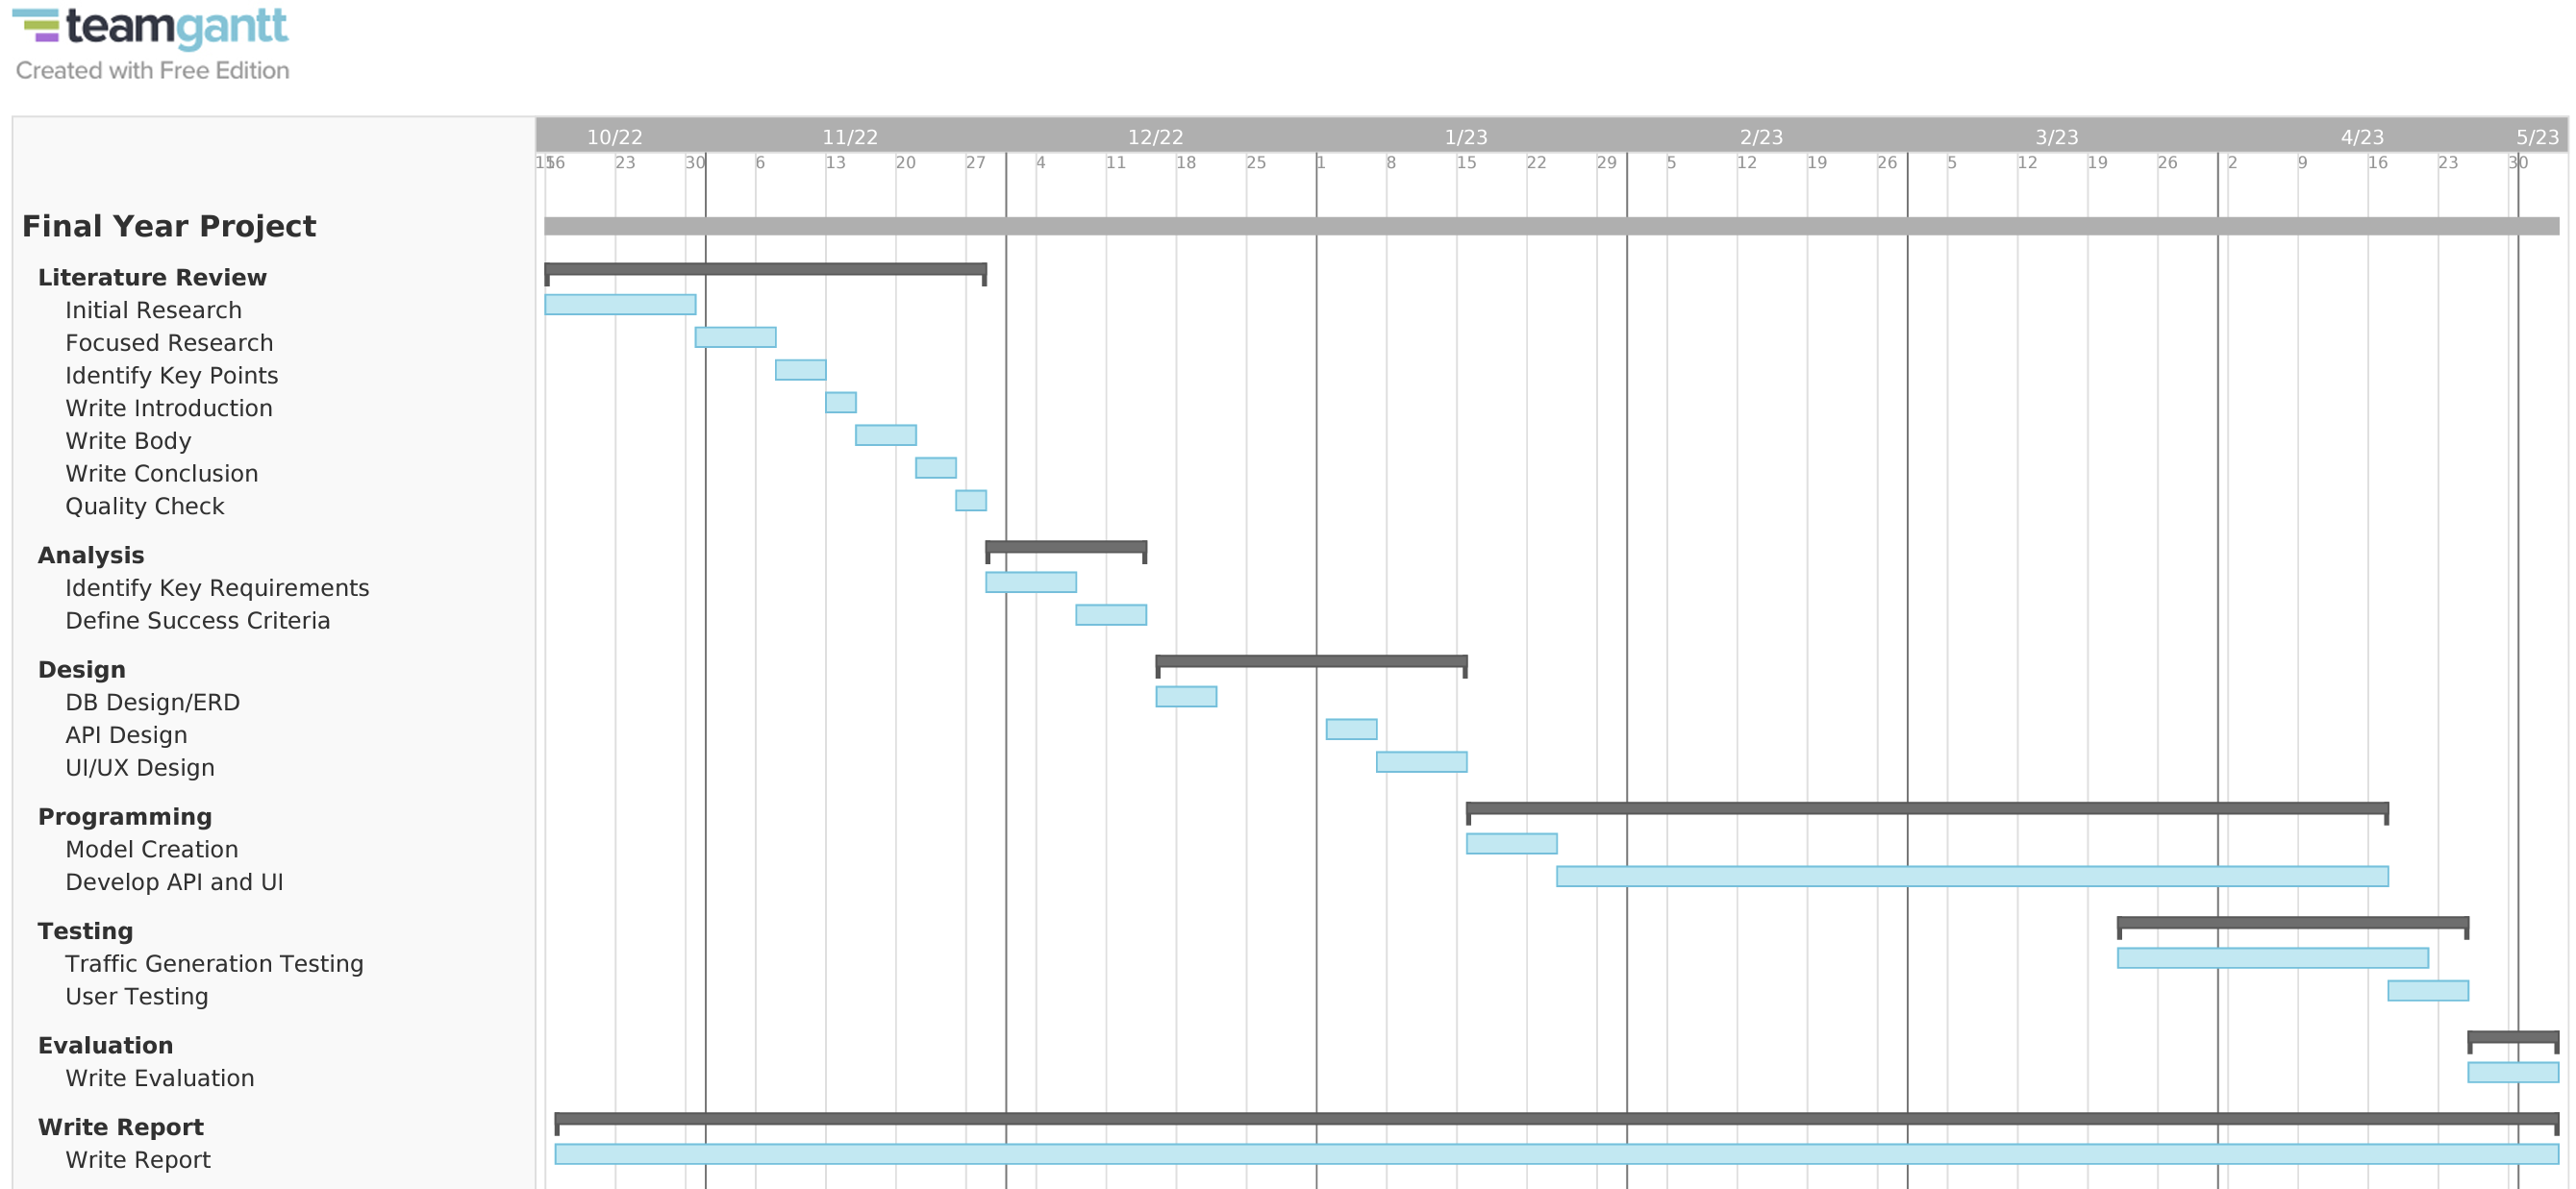
\includegraphics[scale=0.2]{images/gantt-chart.png}
    \caption{Gantt chart used to outline the key project milestones}
    \label{fig:gantt-chart}
\end{figure}
As the project will follow the Kanban development methodology, some stages overlap and will occur simultaneously. This is because testing will be critical to influencing the development process and ensuring that features work correctly as they are developed. The tight timescale of this project also means that tight features be tested as they are written to prevent issues later in the project.
\section{Project Management}
\label{methodology:project-management}
To ensure secure storage, accessibility and history of code as it is written, Git will be used to manage the project. Git is a version control system that allows for the tracking of changes to code and the ability to revert to previous versions of the code. GitHub will be used to host the code and will allow for the code to be accessed from anywhere, GitHub also has a free tier which will be used for this project. The GitHub repository for this project can be found at \url{https://github.com/mattg66/fyp}.
\chapter{Requirements}
\label{chap:requirements}

This chapter will provide detail on the requirements for the automation
platform. The requirements will be split into 2 sections, namely the functional
requirements and non-functional requirements. The functional requirements
will outline the features that the platform must have and the non-functional
requirements will outline the requirements that the platform must meet to be successful.
To prioritise the requirements, the MoSCoW method will be used. This method will allow for the requirements to be prioritised and will ensure that
the most important requirements are met first. The MoSCoW method is a
prioritisation method that splits requirements into 4 categories, namely: Must
Have, Should Have, Could Have and Won’t Have.
\section{Functional Requirements}
Functional requirements are outlined by the IEEE as a ``function that a system or system component must be able to perform''. \citep{159342}

\begin{center}
    \begin{table}[H]
        \begin{tabular}{l p{0.6\linewidth} l}
            \hline
            \textbf{ID} & \textbf{Details}
                        & \textbf{Priority}
            \\ \hline
            FR1         & Visual representation of rack space
                        & Must Have
            \\ \hline
            FR2         & Add and remove racks from the space
                        & Must Have
            \\ \hline
            FR3         & Add and remove Terminal Servers from racks
                        & Must Have
            \\ \hline
            FR4         & Add and remove Fabric Nodes from racks
                        & Must Have
            \\ \hline
            FR5         & Add, remove and update projects
                        & Must Have
            \\ \hline
            FR6         & Expand or contract a projects consumption of rack
            space       & Must Have
            \\ \hline
            FR7         & Automate configuration of ACI fabric
                        & Must Have
            \\ \hline
            FR8         & Deploy virtual router using vCenter API
                        & Must Have
            \\ \hline
            FR9         & Deploy virtual services stack to provide remote
            access VPN  & Could
            Have
            \\ \hline
            FR10        & Continuous monitoring of ACI and vCenter health
                        & Won’t Have
            \\
            \hline
            FR11        & Terminal server automated management
                        & Must Have
            \\ \hline
            FR12        & Login system to restrict access                   & 
            Could Have                                                         \\
        \end{tabular}
        \caption{Functional Requirements}
        \label{requirements:functional}
    \end{table}
\end{center}

FR1 - FR2 outlines the requirements to have the rack space visualised in the web application of the solution. The idea behind this is that the application will simplify the process of adding and removing racks which will allow for the rack space to be easily recreated, and will also allow for the rack space to be easily updated if the rack space changes.
It will also help show the utilisation of the space, and allow for project planning to be carried out more easily.

FR3 - FR4 outlines the ability to associate \gls{aci} nodes and terminal servers to racks, this is required so that the automation backend can push the required config out when a rack is onboarded into a project. This also adds the ability to add and remove nodes and terminal servers if any physical changes occur in the rack space.

FR5 details the ability of the automation platform to store projects. This will provide the core functionality of the platform, where the current projects are stored and managed through the automation platform.

FR6 details the requirement to expand and contract a project's rack space utilisation, this will allow for the project to be scaled up or down as required which is a common occurrence.

FR7 outlines the core automation functionality of the platform. This is to automate the deployment of connectivity to the \gls{aci} fabric based on the selected rack space and associated fabric nodes.

FR8 outlines the deployment of a virtual router to the vCenter automation platform. This will provide internet connectivity to the project network created by FR7.

FR9 provides the ability to automate the creation of a project services stack, this may include services such as \gls{vpn} and \gls{ntp} to name a few.

FR10 outlines the possibility of having continuous status monitoring of ACI and vCenter, however, due to the required time to implement this feature it has been marked as a Won’t Have.

FR11 details the ability to also automate the terminal servers associated with racks which will ensure that terminal servers are connected to projects upon their onboarding.

FR12 details the possibility of implementing a login system, whilst this would be a useful feature and should be implemented at some point, the project will be hosted on a secure network that requires access to be granted, so the login system may be out of scope given the time restrictions.
\section{Non-Functional Requirements}
Non-functional requirements describe the non-behavioral characteristics of a system, capturing the properties and constraints under which a system must operate \citep{12} 
\begin{center}
    \begin{table}[H]
        \begin{tabular}{l p{0.6\linewidth} l}
            \hline
            \textbf{ID}             & \textbf{Details}
                                    & \textbf{Priority}
            \\ \hline
            NFR1                    & Must be easy to use for staff with less technical
            knowledge
                                    & Must Have
            \\ \hline
            NFR2                    & The system status should be easily visible to staff (e.g.
            errors, project status) & Must Have                                                                                       \\ \hline
            NFR3                    & The system should be able to easily integrate with existing \gls{aci} fabric deployments & Could have
        \end{tabular}
        \caption{Non-Functional Requirements}
        \label{requirements:non-functional}
    \end{table}
\end{center}

NFR1 outlines the requirement for the web application to be easy to use for less experienced team members. Through the use of abstraction, the networking and configuration can be hidden behind an easy to use web interface through the use of automation scripts that are run as a result of the user's actions.

NFR2 shows that the system must report the status to staff via the use of status indicators. This should show the progress of the automation scripts as they progress through automating and applying the configuration to various elements of the network.

NFR3 outlines for the platform to be able to integrate with existing \gls{aci} fabric deployments. This will allow for the platform to be used in a production environment without the need to reconfigure and rearchitect the fabric. Ideally, the platform should be deployed alongside a new fabric in a greenfield deployment.



%%%%%%%%%%%%%% REFERENCES SECTION
\newpage
\phantomsection
\addcontentsline{toc}{chapter}{References}
% In order to try and get a consistent format I copy and paste the INSPIRE bibtex code into my bibtex file.
\printbibliography
%%%%%%%%%%%% Include your appendices here


\end{document}